\section{Landing Strategy}

\begin{figure}[ht]
\center
  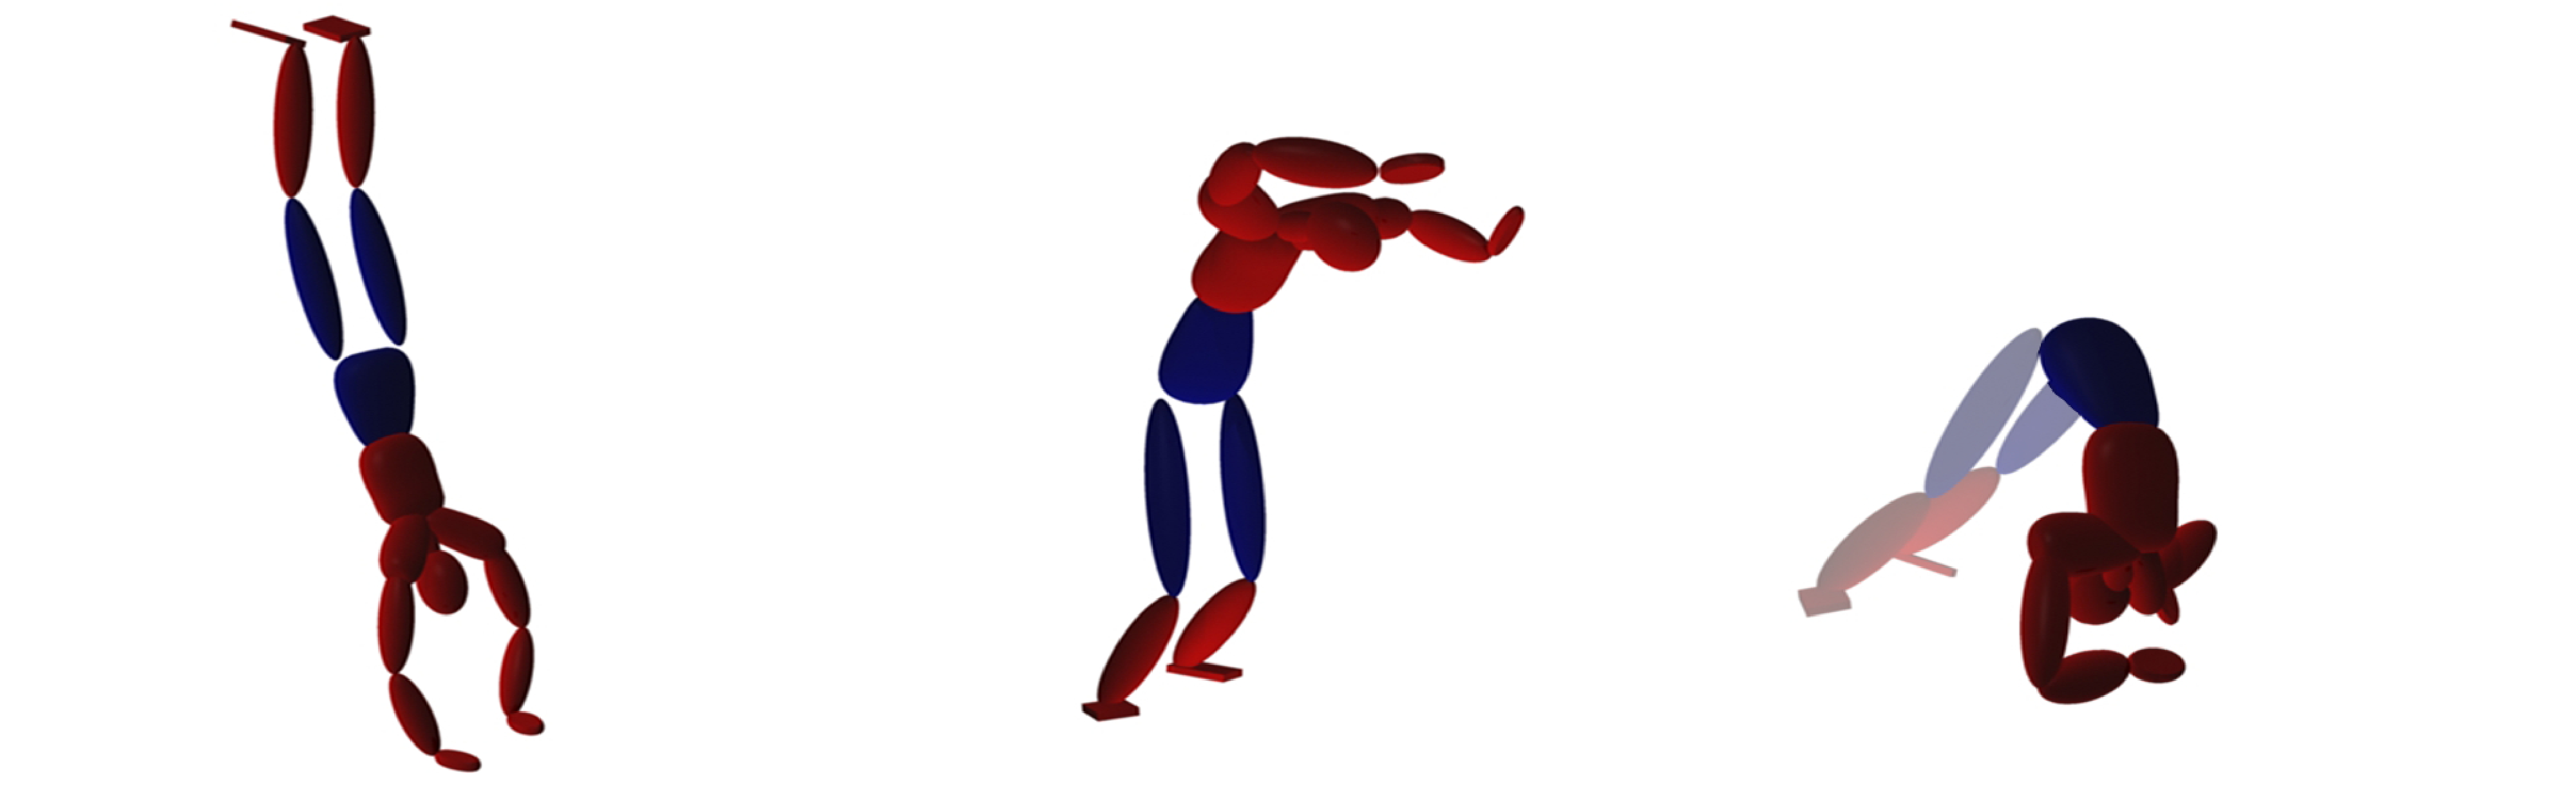
\includegraphics[width=3.2in]{images/LandingPoses}
  \caption{
    The left and middle are the desired landing poses for the
    hands-first strategy and the feet-first strategy, respectively.
    The right is the ready-to-roll pose for the feet-first strategy,
    which we track only the upper body.
  }
 \label{fig:landing_landingPoses}
\end{figure}

Given an initial condition at the beginning of a fall, the character
can choose to land with the hands-first strategy or the feet-first
strategy.  In general, the hands-first strategy is chosen only for
aesthetics purpose because it is less robust and suitable only for
falls with planar angular momentum (about the pitch axis). In
contrast, the feet-first strategy can handle a wide range of arbitrary
initial conditions because it includes an extensive foot-ground
contact duration to modulate the momentum before rolling. A
landing strategy also includes a desired landing pose. Our algorithm
only requires a partial pose to stretch the arms or legs at landing,
depending on whether the hands-first or the feet-first strategy is
chosen. We manually specify this partial pose for each strategy
(\figref{landing_landingPoses}).

\begin{figure}[0.3\textwidth]
  \begin{center}
    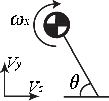
\includegraphics[width=0.28\textwidth]{images/COM}
  \end{center}
  \caption{Landing condition variables.}
  \label{fig:landing_com}
\end{figure}

An integral part of our landing strategy is the landing condition, a
simple equation that compactly characterizes successful landing
motions.
\ignorethis{ A landing strategy describes an ideal landing
  condition key to the success of the subsequent rolling motion. We
  wish to derive a simple equation that compactly characterizes
  successful landing motions.} If the character manages to turn a fall
into a roll and gets back on its feet at the end of the roll, we
consider it successful.  Because a successful landing highly depends
on whether the character is able to control the momentum
at the moment of the first contact ($T$),
%% the character's momentum at the moment of first contact ($T$), 

our algorithm defines the landing condition as a relation between the
global linear velocity $\vc{v}^{(T)}$, global angular velocity
$\vc{\omega}^{(T)}$, and the angle of attack $\theta^{(T)}$, which
approximates the global orientation of the character
(\revised{\figref{landing_com}}).
The actual
coefficients of the landing condition depend on the design of the
landing controller, which cannot be derived analytically, but can be
learned from examples generated by the landing controller. We apply a
sampling method, similar in spirit to the approach Coros \etal
\cite{Coros:2009:RTC} presented for biped locomotion, to determine the
landing condition for a particular landing strategy.  \ignorethis{ A
  successful landing also depends on the design of the landing
  controller, which cannot be expressed in an analytical form.
  Therefore, we use a sampling approach to derive the relation,
  similar in spirit to the approach Coros \etal \cite{Coros:2009:RTC}
  presented for biped locomotion.}

\begin{figure}[ht]
\center
  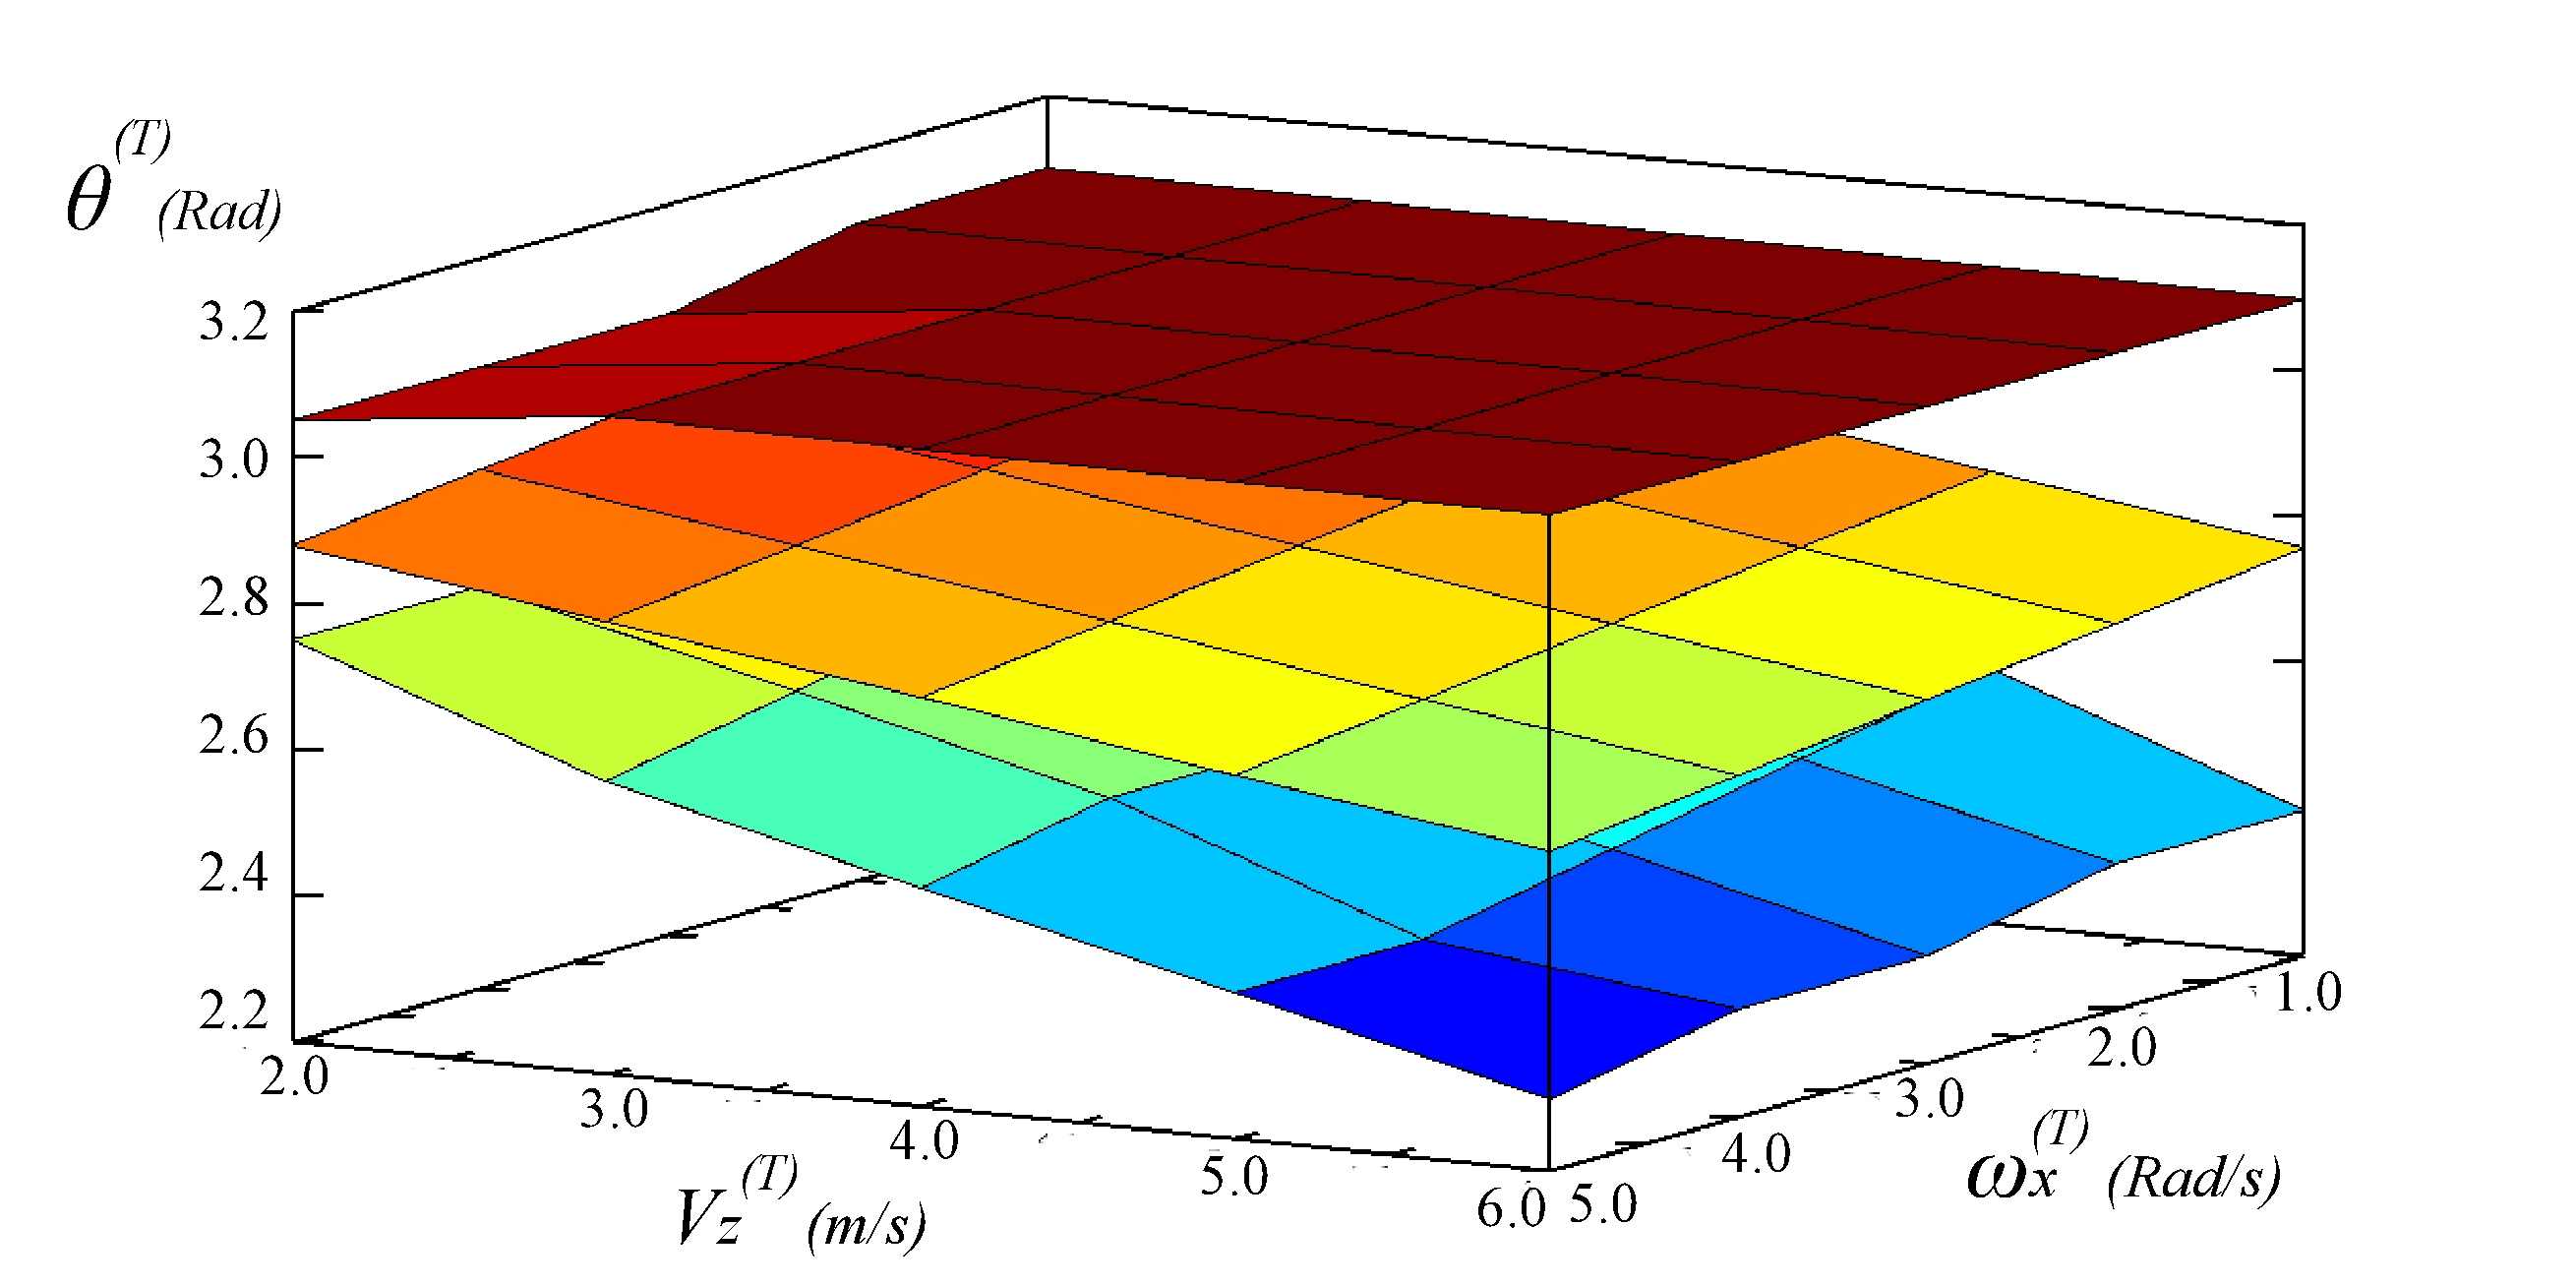
\includegraphics[width=0.49\textwidth]{images/sampleVZWX}
  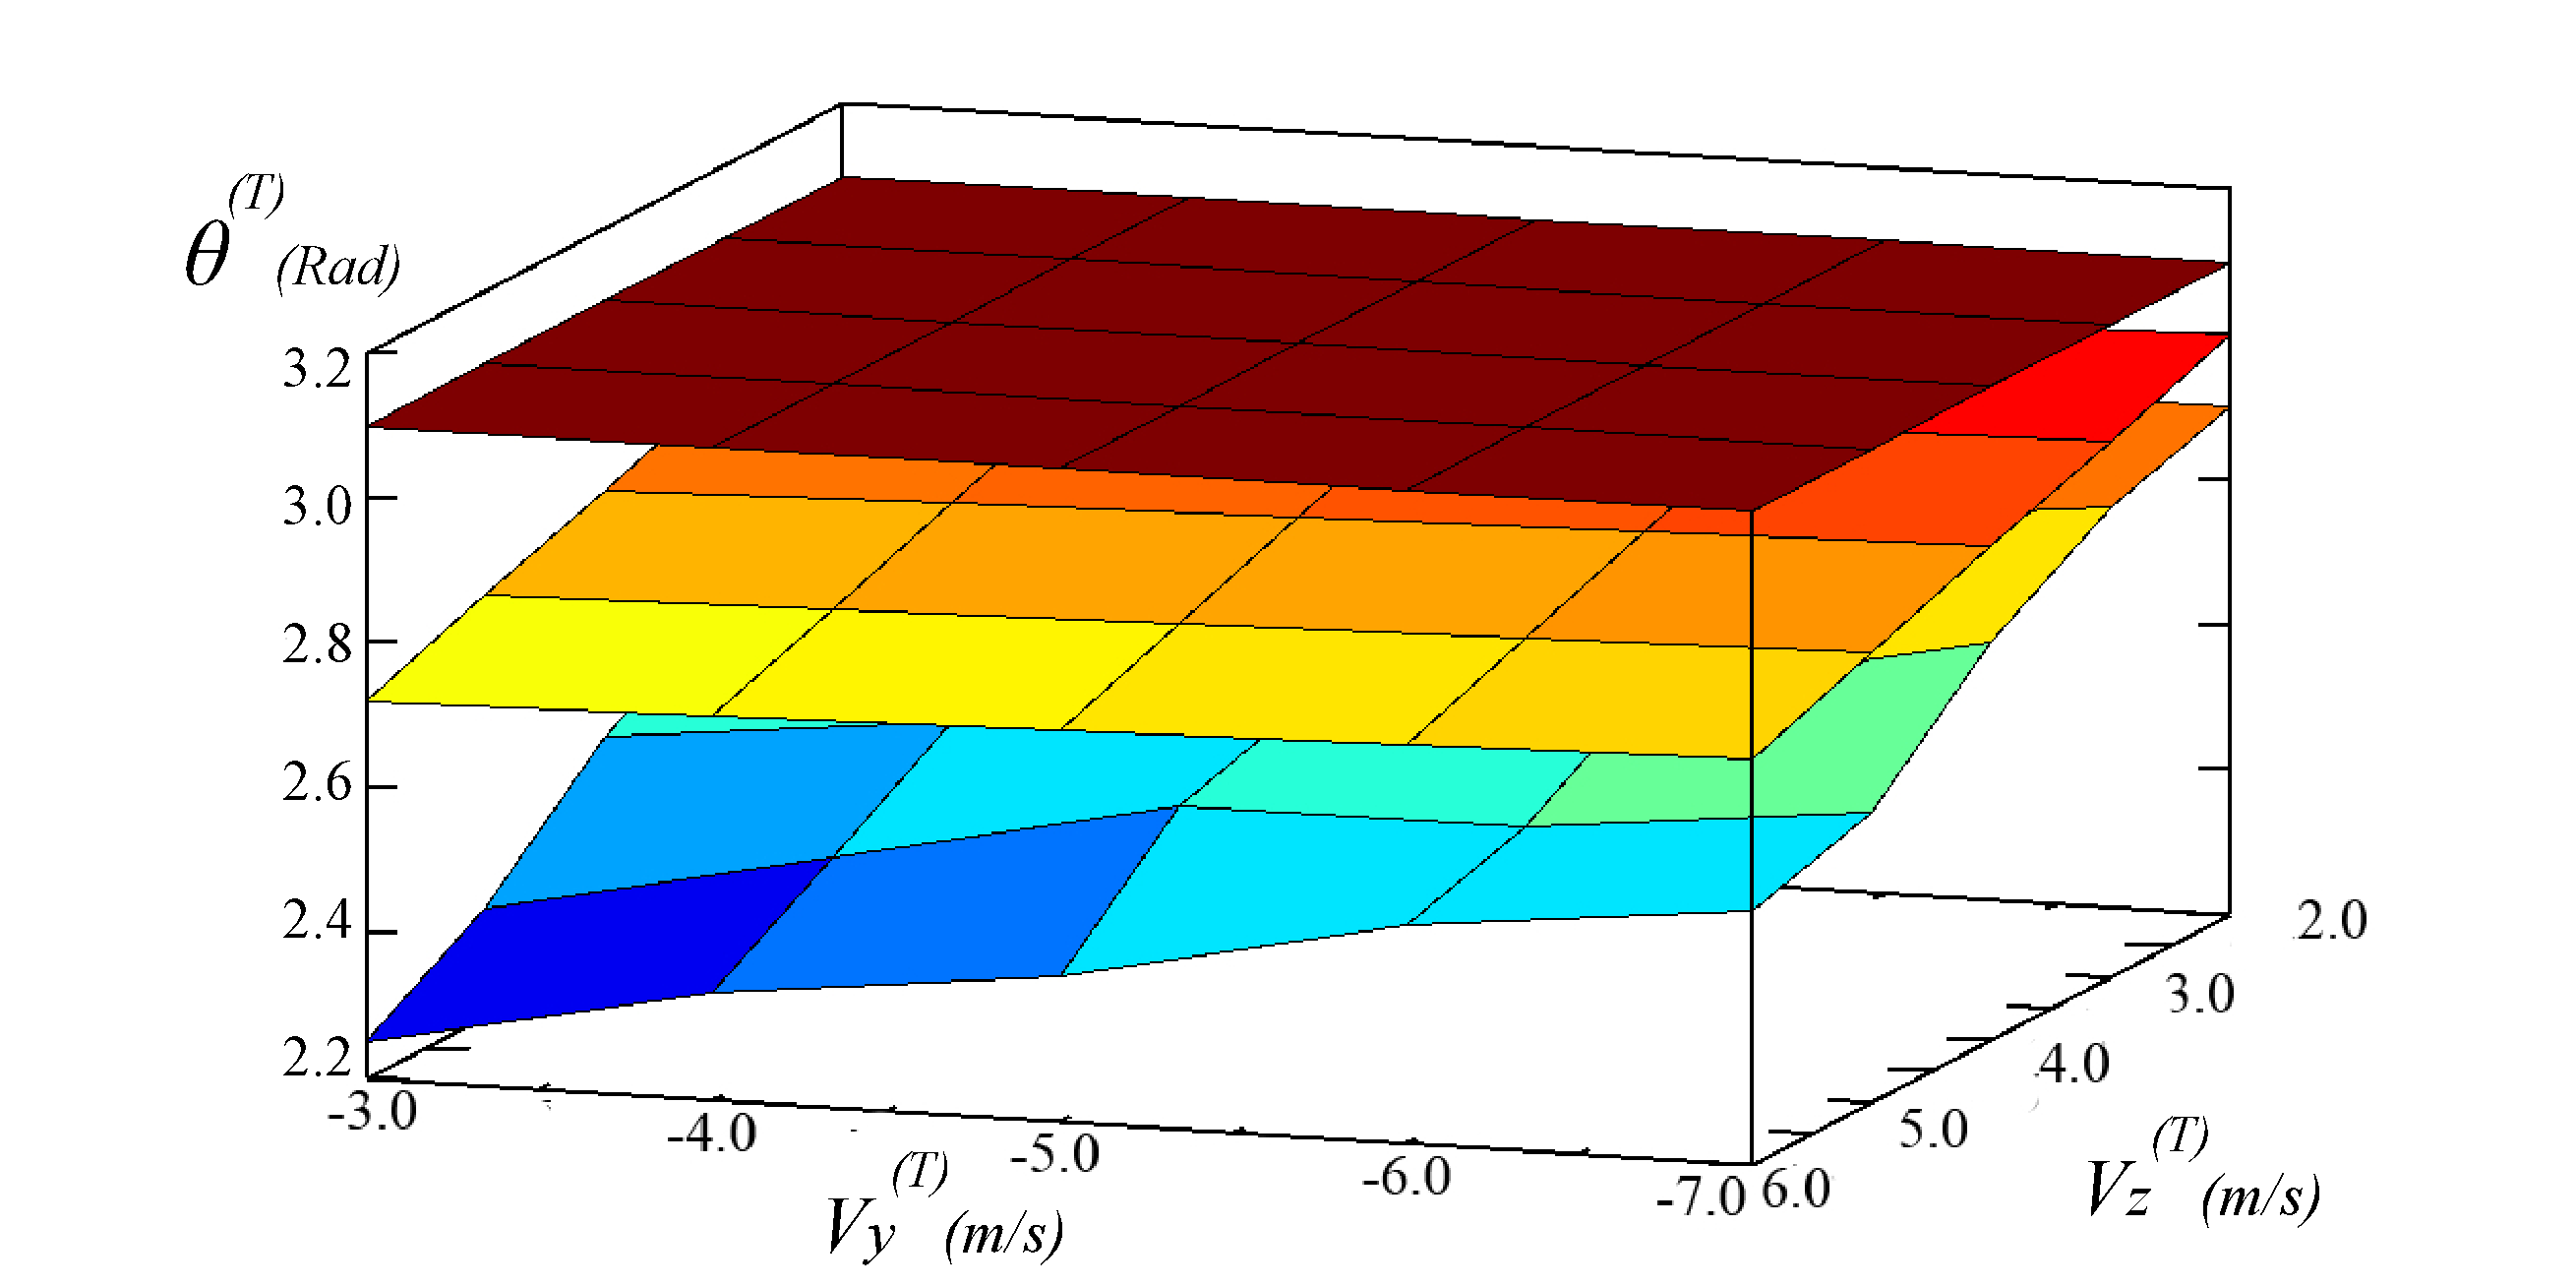
\includegraphics[width=0.49\textwidth]{images/sampleVYVZ}
  \caption{
    Samples for hands-first landing strategy. Successful samples are
    bounded between top and bottom planes along $\theta^{(T)}$
    axis. The middle plane, average of the two, indicates the linear
    relation of the ideal landing condition. 
  }
\ignorethis{
\emph{Top}: x-axis: 
    Domain spanned by $v_z^{(T)}$, $\omega_x^{(T)}$ and $\theta^{(T)}$ \emph{(Top)}
    Domain spanned by $v_z^{(T)}$, $v_y^{(T)}$ and $\theta^{(T)}$ \emph{(Bottom)}
  }
 \label{fig:landing_samplesPlanar}
\end{figure}
 
For the hands-first strategy with planar motion, we consider a
four-dimensional space spanned by $\theta^{(T)}$, $v_y^{(T)}$,
$v_z^{(T)}$ and $\omega_x^{(T)}$. Given a sample in the parameter
space, we run our landing controller to test whether the character can
successfully get up at the end. Empirical results from thousands of
random samples show that the successful region is mostly continuous
and linear (Figure \ref{fig:landing_samplesPlanar}). We can bound the
successful samples in the $\theta^{(T)}$ axis using two hyperplanes.
Taking the average of the maximum and the minimum planes, we derive a
linear relation between the angle of attack and the landing velocities as
\begin{equation}
\label{eqn:landing_approxLandingAngle}
\theta ^{(T)} = a \;v_y^{(T)} + b \;v_z^{(T)} + c \;\omega_x^{(T)} + d
\end{equation}
where $a$, $b$, $c$, and $d$ are the coefficients of the fitted
hyperplane. Note that Equation (\ref{eqn:landing_approxLandingAngle}) is a
sufficient but not necessary condition for successful landing. Most
points between the maximal and minimal hyperplanes also lead to
successful landing motions. This means that even when the character
cannot meet the landing condition exactly, it still has a good chance
to land successfully. For the feet-first strategy, in theory, we need
to consider all six dimensions of linear velocity and angular
velocity. However, our empirical results show that non-planar
velocities do not affect $\theta^{(T)}$ as long as they stay within a
reasonable bound (Figure \ref{fig:landing_sampleNonPlanar}). As a result, the
feet-first strategy is able to handle non-planner falling motion using
the same parameters (but different coefficients) in Equation
(\ref{eqn:landing_approxLandingAngle}).

\begin{figure}[ht]
\center
  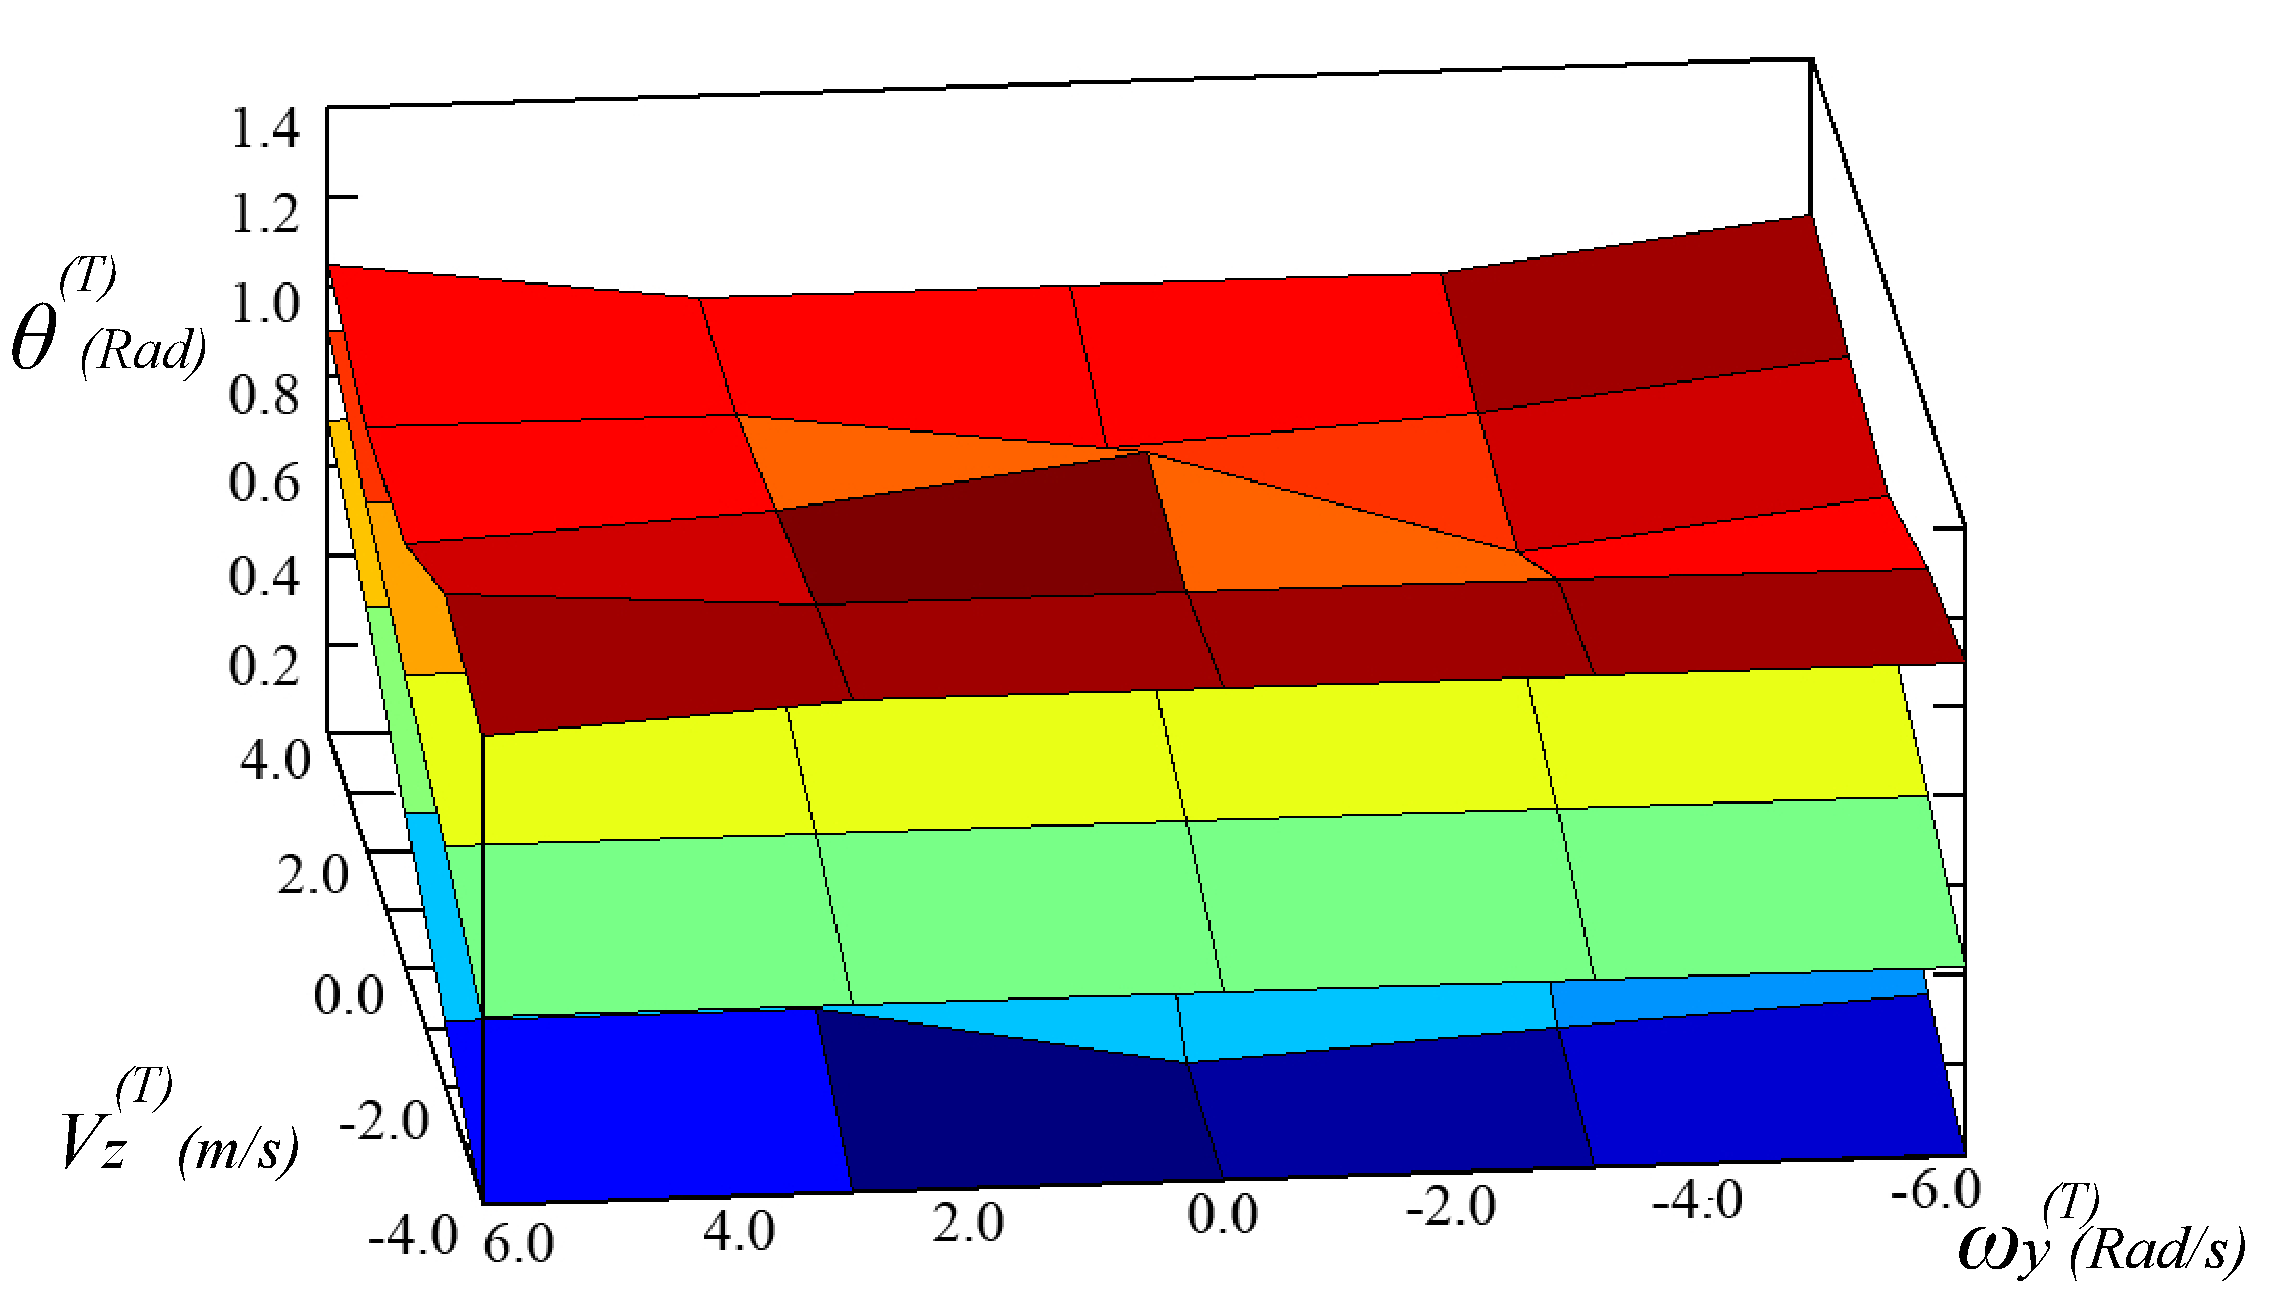
\includegraphics[width=0.51\textwidth]{images/sampleWYflat}
  \caption{
    Samples in the space of $v_z^{(T)}$, $\omega_y^{(T)}$, and
    $\theta^{(T)}$. The spinning velocity $\omega_y^{(T)}$
    has minimal effect on the success of a sample.
  }
 \label{fig:landing_sampleNonPlanar}
\end{figure}


\section{Airborne Phase}
Once the character decides on a landing strategy, the goal of the
airborne phase is to achieve the corresponding landing pose and
landing condition. Because momentum is conserved in air, the linear
velocity, the total airborne time $T$, as well as the angular momentum
are already determined by the initial condition of the fall.  However,
the character can still control the angular velocity $\omega_x^{(T)}$
and the angle of attack $\theta^{(T)}$ by varying its pose (\ie
actuated degrees of freedom (DOFs) excluding the global position and
orientation) to change the moment of inertia. To most effectively
achieve the desired landing condition, we design our airborne
algorithm based on the strategy employed in platform diving
competition, where a highly trained athlete performs a sequence of
predefined poses to manipulate the final orientation and angular
velocity.

To this end, our airborne controller uses a PD servo to track a
sequence of poses that lead to the ideal landing condition. 
The sequence of poses is replanned frequently to correct the errors
caused by perturbation and numerical approximation. Each time the
algorithm makes a new plan, an optimal sequence of poses from the
current moment to the landing moment is computed. This sequence
starts with the current pose $\vc{q}_0$ and ends at the desired
landing pose $\vc{q}_T$ (determined by the landing strategy), with a
duration of $T$ seconds. Our control algorithm searches for an
intermediate pose $\vc{q}^*$ and a duration $\Delta t^*$, such that
the character can reach the ideal landing condition by changing to
$\vc{q}^*$ immediately and holding the pose $\vc{q}^*$ for $\Delta
t^*$ seconds before changing to the final pose $\vc{q}_T$.

We formulate an optimization to solve for an intermediate pose $\vc{q}$
and its holding duration $\Delta t$ that can best achieve the ideal
landing condition. The cost function  $g(\vc{q}, \Delta t)$ is defined
in Equation \ref{eqn:landing_landingCondition}.

\begin{equation}
g(\vc{q}, \Delta t) = \theta^{(T)}(\vc{q}, \Delta t) - a \;v_y^{(T)} - b \;v_z^{(T)} - c\;
\omega_x^{(T)}(\theta^{(T)}) - d
\label{eqn:landing_landingCondition}
\end{equation}
Note that $\omega_x^{(T)}$ is a function of $\theta^{(T)}$ because we
need global orientation of the character at time $T$ to compute the
global angular velocity. If we can compute $\theta^{(T)}$, Equation
(\ref{eqn:landing_landingCondition}) can be readily evaluated. Unfortunately,
for a complex 3D multibody system, an analytical solution for
$\theta^{(T)}$ is not available. We could resort to numerical
simulation of the entire airborne phase, in which the character goes
through $\vc{q}_0$, $\vc{q}^*$, and $\vc{q}_T$ subsequently. However,
involving forward simulation of a full skeleton in the cost function
is too costly for our real-time application.\ignorethis{However, we
  cannot compute $\theta^{(T)}$ analytically and have to resort to
  numerical simulation of the entire airborne phase, in which the
  character goes through $\vc{q}_0$, $\vc{q}$, and $\vc{q}^T$
  subsequently. Such simulation of a full skeleton is too costly for a
  real-time application.} Instead, we simulate a simple proxy model
with only six DOFs. When the character is holding a pose, the proxy
model behaves like a rigid body with a fixed inertia.  When the
character transitions from one pose to another, we assume the inertia
of the proxy model changes linearly within a fixed duration $\Delta
t_C$ ($\Delta t_C = 0.1s$ in our implementation). By simulating the proxy
model for the duration of $T$, we obtain the angle of attack
$\theta^{(T)}$ and angular velocity $\omega^{(T)}$ as
follows.
\begin{eqnarray}
\vc{R}(\theta^{(T)}) = \vc{R}(\theta^{(0)}) + \int_{t=0}^{\Delta t_c}
[\vc{I}^{-1}_{A}(t)\vc{L}]\vc{R}(\theta^{(t)}) dt \nonumber \\ 
+ \int_{t=\Delta t_c}^{\Delta t_c + \Delta
  t}[\vc{I}^{-1}(\vc{q},\theta^{(t)})\vc{L}]\vc{R}(\theta^{(t)}) dt \nonumber \\ + \int_{t=\Delta
  t_c+\Delta t}^{2 \Delta t_c + \Delta t}
[\vc{I}^{-1}_{B}(t)\vc{L}]\vc{R}(\theta^{(t)}) dt \nonumber \\ +
\int_{t=2 \Delta t_c+\Delta t}^T
[\vc{I}^{-1}(\vc{q}_T,\theta^{(t)})\vc{L}]\vc{R}(\theta^{(t)}) dt; \\
\omega^{(T)} = \vc{I}^{-1}(\vc{q}_T,\theta^{(T)})\vc{L}
\end{eqnarray}
where $\vc{R}$ is the rotation matrix, $\vc{I}(\vc{q})$ is an inertia
matrix evaluated at pose $\vc{q}$, and $\vc{L}$ is the angular
momentum. $\vc{I}_{A}(t)$ is an interpolated inertia matrix between $\vc{I}(\vc{q}_0)$ and
$\vc{I}(\vc{q})$, and similarly, $\vc{I}_{B}(t)$ is an interpolated matrix between
$\vc{I}(\vc{q})$ and $\vc{I}(\vc{q}_T)$. The operator $[\;]$ represents the skew
symmetric matrix form of a vector.

% \ignorethis{
% an airborne character can
% only control its pose (\ie actuated degrees of freedom) to change
% the moment of inertia, but cannot directly control the global position and orientation. To this end, we design an airborne controller that
% determines a sequence of poses and uses proportional-derivative (PD)
% servos to track them. In our problem, the initial pose $\vc{q}_0$ is
% determined by the initial conditions of the fall, and the final pose
% $\vc{q}_T$ is determined by the landing strategy. Our algorithm,
% therefore, searches for an intermediate pose $\vc{q}^*$ from a
% predefined pose set and a duration $\Delta t^*$ such that the
% character can achieve the ideal landing condition by changing from
% $\vc{q}_0$ to $\vc{q}^*$ immediately after the fall begins, holding
% $\vc{q}^*$ for $\Delta t^*$ seconds, and changing to $\vc{q}_T$ until
% the end of airborne phase.

% To search for the optimal control parameters, $\vc{q}^*$ and $\Delta
% t^*$, we need to define a cost function, $g(\vc{q}, \Delta t)$ which
% evaluates how well the falling motion achieves the ideal landing
% condition for a given estimate of control parameters. We will first
% describe how we derive landing conditions, followed by the details of
% the search algorithm.


% \paragraph{Search for optimal control parameters.}
% Using the derived landing condition, we now define the cost function
% as

% \begin{equation}
% g(\vc{q}, \Delta t) = \theta^{(T)}(\vc{q}, \Delta t) - a \;v_y^{(T)} - b \;v_z^{(T)} - c\;
% \omega_x^{(T)} - d
% \label{eqn:landingCondition}
% \end{equation}

% Due to conservation of momentum and a known final pose, $v_y^{(T)}$,
% $v_z^{(T)}$ and $\omega_x^{(T)}$ can be computed from the initial
% condition of the fall. The only unknown value in Equation
% \ref{eqn:landingCondition} is $\theta^{(T)}$, which depends on the
% control parameters, $\vc{q}$ and $\Delta t$. Because we cannot compute
% $\theta^{(T)}$ analytically, we propose to simulate the entire
% airborne motion, going through the initial pose $\vc{q}_0$, the
% estimated intermediate pose $\vc{q}$, and the final pose $\vc{q}_T$,
% subsequently.

% However, simulating a full skeleton is too costly for efficient
% evaluation of $g(\vc{q}, \Delta t)$. Instead, we simulate a simple
% model with only six DOFs as a rigid body, but we allow its inertia to
% vary over time. When the character transitions from one pose to
% another, we assume the inertia changes gradually within a fixed
% duration $\Delta t_C$. The angle of attack for the simple model can be
% expressed as following equation and integrated numerically:
% \begin{eqnarray}
% \vc{R}(\theta^{(T)}) = \vc{R}(\theta^{(0)}) + \int_{t=0}^{\Delta t_c}
% [\vc{I}^{-1}(\vc{q}_A(t))\vc{L}]\vc{R}(\theta^{(t)}) \nonumber \\ 
% + \int_{t=\Delta t_c}^{\Delta t_c + \Delta
%   t}[\vc{I}^{-1}(\vc{q})\vc{L}]\vc{R}(\theta^{(t)}) \nonumber \\ + \int_{t=\Delta
%   t_c+\Delta t}^{2 \Delta t_c + \Delta t}
% [\vc{I}^{-1}(\vc{q}_B(t))\vc{L}]\vc{R}(\theta^{(t)}) \nonumber \\ +
% \int_{t=2 \Delta t_c+\Delta t}^T [\vc{I}^{-1}(\vc{q}_T)\vc{L}]\vc{R}(\theta^{(t)})
% \end{eqnarray}
% where $\vc{R}$ is the rotation matrix, $\vc{I}(\vc{q})$ is an inertia
% matrix evaluated at pose $\vc{q}$, and $\vc{L}$ is the angular
% momentum. $\vc{q}_A(t)$ is an interpolated pose between $\vc{q}_0$ and
% $\vc{q}$, and similarly, $\vc{q}_B(t)$ is an interpolated pose between
% $\vc{q}$ and $\vc{q}_T$. The operator $[\vc{a}]$ is the skew symmetric
% matrix of a vector $\vc{a}$.
% }
% \ignorethis{
% To interpolate the inertia, inertia matrices are decomposed into a rotation matrix
%  $\mat{R}$ and a axis-aligned matrix $\mat{I_A}$ using Singular Value Decomposition 
% and interpolated using slerp and weighted sum. 

% \begin{eqnarray}
% \mat{I_0} = \mat{R_0} \mat{I}_{A0} \mat{R_0}^T \nonumber \\
% \mat{I_1} = \mat{R_1} \mat{I}_{A1} \mat{R_1}^T \nonumber \\
% \mat{R}(w) = slerp(\mat{R_0}, \mat{R_1}, w) \nonumber \\
% \mat{I}(w) = \mat{R}(w) (w \mat{I}_{A0} + (1-w)\mat{I}_{A1}) \mat{R}(w)^T \nonumber
% \end{eqnarray}

% While inertia is updated, angular velocity should be updated as well
% to preserve angular momentum. A rigid body simulation is relatively
% inaccurate comparing to the full simulation, but it is enough to
% approximate the landing angle $\theta(T)$ as shown in Figure
% \ref{fig:inertiaTrajectory}. After the simulaton ended, the cost
% functions returns the difference between the current orientation and
% the desired landing angle of attack $\theta(T)$.  
% }

% %% \sehoon{
To formulate an efficient optimization for real-time application, we
represent the domain of intermediate pose as a finite set of candidate
poses, instead of a continuous high-dimensional Euclidean space. This
simplification is justified because a handful of poses is sufficient
to effectively change the moment of inertia of the character. As a
preprocess step, our algorithm automatically selects the candidate set
$\mat{Q}$ from a motion capture sequence in which the subject performs
range-of-motion exercise. The selection procedure begins with a seed
pose $\bar{\vc{q}}_0$ and increments the set by adding a new pose
$\bar{\vc{q}}_{new}$ which maximizes the diversity of inertia
(Equation \ref{eqn:landing_selectingCandidate}). In our experiment, 16 poses
are sufficient to present a variety of moment of inertia
(Figure \ref{fig:landing_candidatePoses}).



% \ignorethis{ The intermediate pose is chosen from a set of predefined
%   poses $\mat{Q}=\{\vc{q}^*_0, \vc{q}^*_1, ... \}$ that can most
%   effectively change each of the six values of the full-body inertia
%   (Figure \ref{fig:candidatePoses}).  We select the set $\mat{Q}$
%   automatically from the captured range of motion.  We start from a
%   selected seed pose $\vc{q}^*_0$ and increment the set by adding a
%   new pose $q^*_{new}$ which maximizes the diversity of inertia
%   (Equation \ref{eqn:selectingCandidate}).  In our experiment, 16
%   poses are compact but sufficient to handle a wide range of initial
%   conditions.}
% %% }

\begin{equation}
\label{eqn:landing_selectingCandidate}
\bar{\vc{q}}_{new} = \argmax_{\vc{q} \in M} (\min_{\bar{\vc{q}}_j \in Q} \| I(\vc{q}) - I(\bar{\vc{q}}_j)\|) \}
\end{equation}
where $M$ contains the poses in the range-of-motion sequence, $Q$
contains the currently selected candidate poses, and $I(\vc{q})$
computes the inertia of pose $\vc{q}$.

%% During the optimization, we loop over each candidate pose in $Q$. For
To find optimal $\vc{q}^*$ and $\Delta t^*$ for each plan, we start from the current pose as $\vc{q}_0$ and loop over each candidate pose in $Q$. For
each candidate pose $\bar{\vc{q}}_i$, we search for the best $\Delta
t$ such that $g(\bar{\vc{q}}_i, \Delta t)$ is minimized. The search can
be done efficiently using one-dimensional Fibonacci algorithm and the
proxy-model simulation. The optimal intermediate pose $\vc{q}^*$ and
its optimal duration $\Delta t^*$ are used for airborne control.

\begin{figure}[ht]
\center
  %% \includegraphics[width=3.2in]{images/AirbornePoses}
  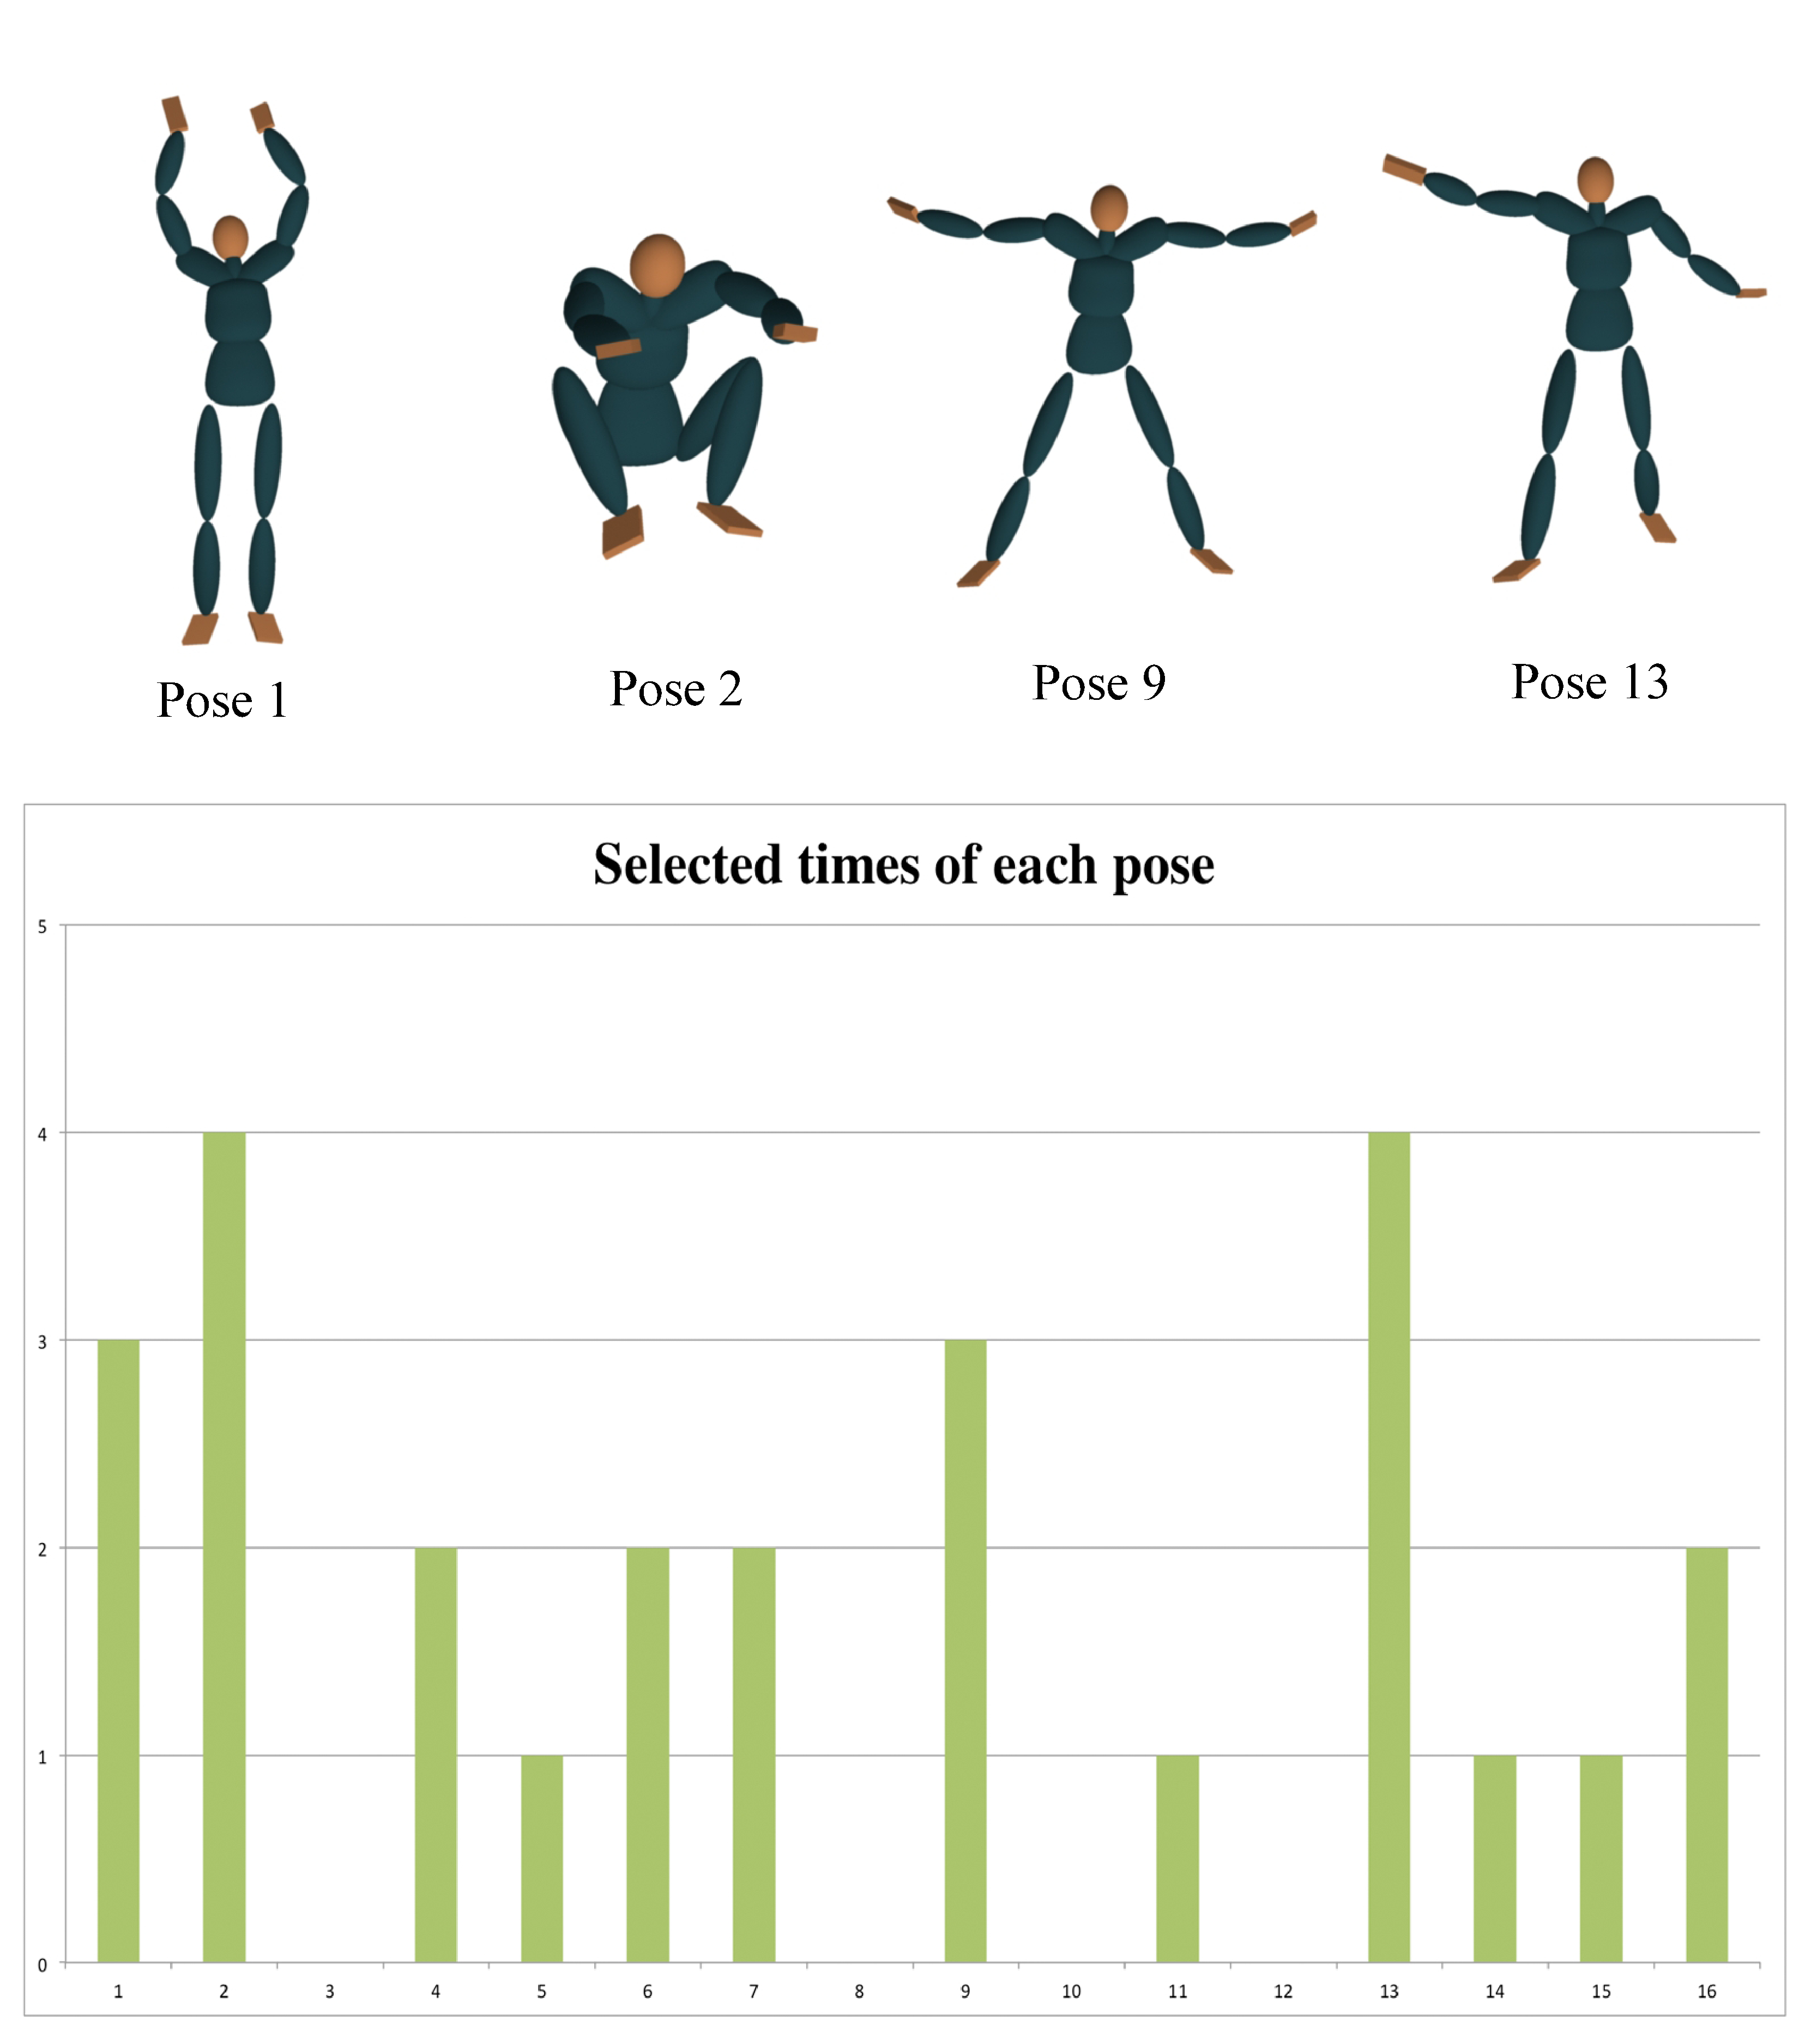
\includegraphics[width=4.2in]{images/PoseWithStats}
  %% \caption{A few popular candidate poses from $\mat{Q}$.
  \caption{
    Among 16 poses in $\mat{Q}$, pose 1, 2, 9, and 13 are frequently 
    selected by the airborne controller
  }
 \label{fig:landing_candidatePoses}
\end{figure}

By design, our algorithm trades off accuracy for efficiency; we use a
fast but less accurate proxy-model simulation and a small set of
predefined poses. Our algorithm is very efficient so that the
character can frequently reassess the situation and replan new poses
to correct any errors or adapt to unexpected perturbations. 

The frequency of replanning can be determined differently for
$\vc{q}^*$ and $\Delta t^*$. In our implementation, we replan
$\vc{q}^*$ at a much lower frequency than $\Delta t^*$ to avoid
unnatural frequent change of poses. In addition, we stop replanning
when the character is within $0.3$ seconds away from the ground.
